\documentclass{article}
\usepackage{graphicx} % Required for inserting images
\graphicspath{ {../diagram/} }
\usepackage[margin=2cm]{geometry}
\usepackage{enumitem}
\usepackage{caption}
\usepackage{subcaption}

\title{DSP in VLSI \\ Homework 2 - Digital Filter}
\author{Jen-Tse Chen}
\date{March 2026}

\begin{document}
\maketitle

\begin{enumerate}
    \item  (Step 1) Please use Matlab/Python to draw the impulse response and frequency response (containing magnitude and phase) of the 25-tap sinc-based FIR filter. Note that you need to use dB scale for the magnitude of the frequency response and use radian for the phase of frequency response versus normalized frequency. The x-axis must be marked with the correct label (20\%). Please explain whether the filter is high-pass, band-pass or low-pass and why. (5\%)

    The impulse response is illustrated in Figure \ref{fig:imp_resp}, while the frequency response—including both magnitude and phase—is presented in Figure \ref{fig:freq_resp}. From the magnitude response, the half-bandwidth is approximately $0.14\pi$ radians. The sawtooth-like artifacts observed in the phase response arise from phase discontinuities at transmission nulls, where the phase is undefined. Based on the overall frequency response characteristics, the filter can be classified as a low-pass filter.

    \begin{figure}[htbp]
        \centering
        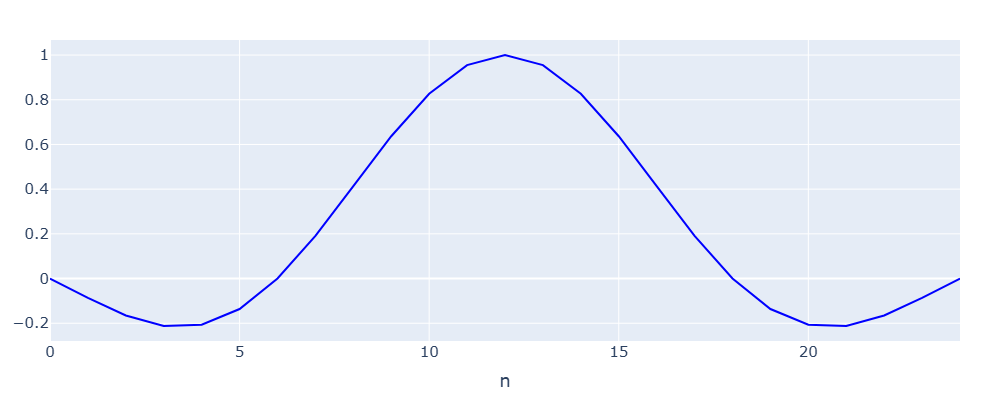
\includegraphics[width=0.8\textwidth]{../diagram/Q1/imp_resp.png}
        \caption{Impulse response}
        \label{fig:imp_resp}
    \end{figure}

    \begin{figure}[htbp]
        \centering
        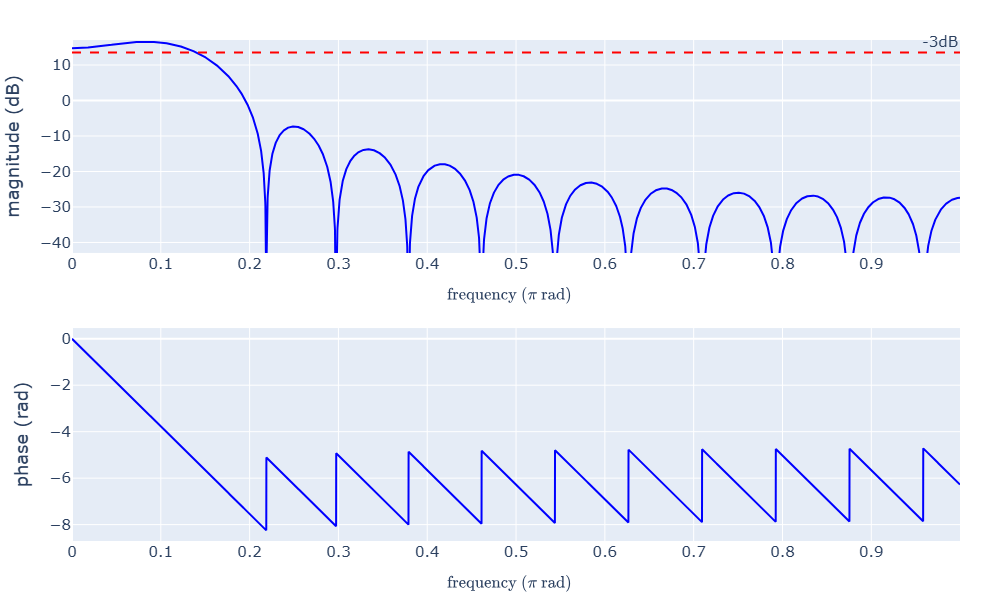
\includegraphics[width=0.8\textwidth]{../diagram/Q1/freq_resp.png}
        \caption{Frequency response}
        \label{fig:freq_resp}
    \end{figure}

    \newpage
    \item (Step 2) Draw the time-domain input and output waveforms after you feed 144 input samples. The filtering effect can be observed. (20\%)
    
    The input signal is shown in Figure \ref{fig:input}, and the corresponding output is presented in Figure \ref{fig:output}. As observed from the figures, the high-frequency components have been effectively attenuated.

    \begin{figure}[htbp]
        \centering
        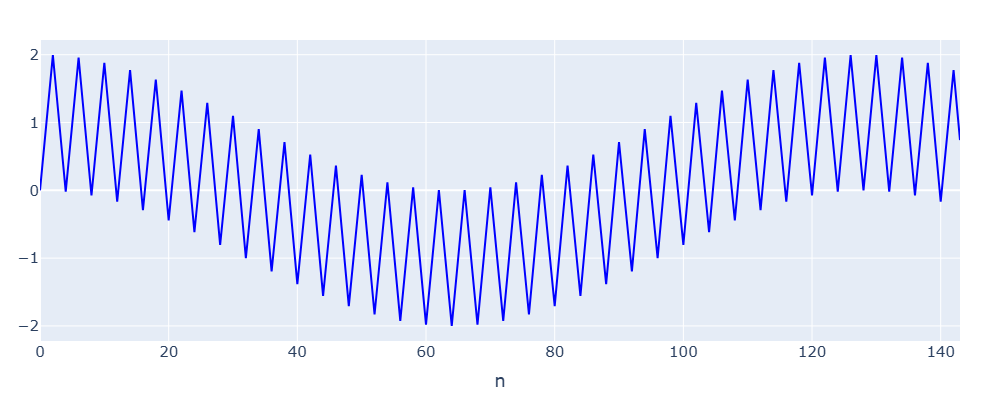
\includegraphics[width=0.8\textwidth]{../diagram/Q2/input.png}
        \caption{Input}
        \label{fig:input}
    \end{figure}
    
    \begin{figure}[htbp]
        \centering
        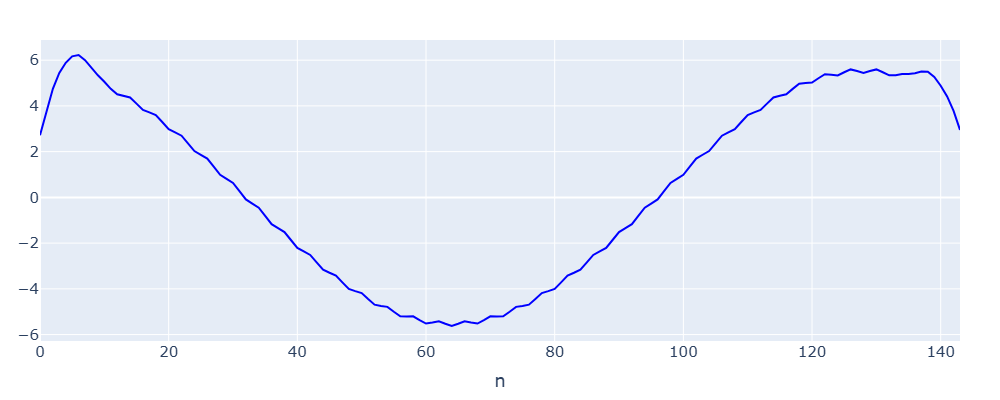
\includegraphics[width=0.8\textwidth]{../diagram/Q2/output.png}
        \caption{Output}
        \label{fig:output}
    \end{figure}

    \newpage
    \item (Step 3) To show how you determine the word-length, please use the word-length of coefficients as the X-axis and error as the Y-axis. Scan the quantization error versus the word-lengths from 9 bits to 15 bits (Four figures each having 7 word-length settings in its x-axis). According the following simulation results, mark the final word-length settings in the block diagram of the direct form FIR filter. (20\%)
        \begin{enumerate}[label=\alph*.]
            \item Output error versus input word-lengths
            \item Output error versus coefficient word-lengths (In this case, the input word-length is fixed to your selected setting.)
            \item Output error versus word-lengths after multiplication (In this case, the input word-length and coefficient word-length are set to your desired value.)
            \item Output error versus word-lengths after addition. (In this case, the fixed-point representations are used for the previous three signals.) 
        \end{enumerate}

        The output RMSE versus input word length is shown in Figure \ref{fig:qntz_input}, while the RMSE versus coefficient word length, multiplier word length, and adder word length are presented in Figures \ref{fig:qntz_coef}, \ref{fig:qntz_mult}, and \ref{fig:qntz_add}, respectively. To satisfy the specification that the RMSE be smaller than $2^{-11}$, the fixed-point format is determined as illustrated in Figure \ref{fig:fixed_point_setting}.

        \begin{figure}[htbp]
            \centering
            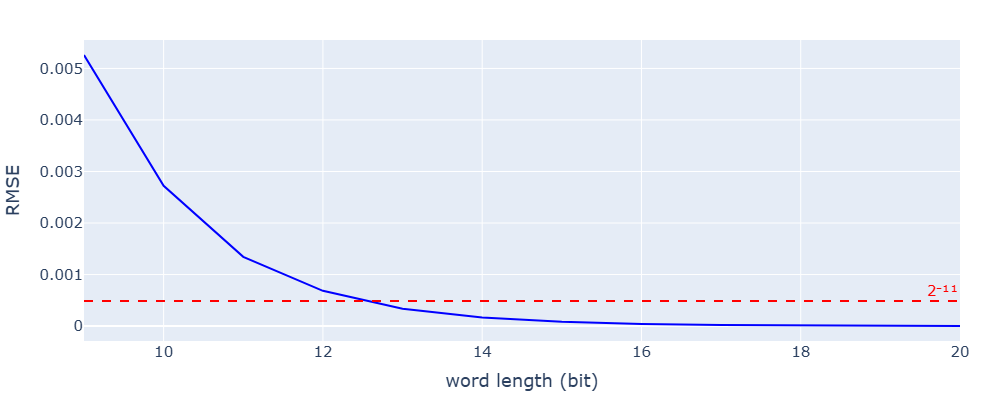
\includegraphics[width=0.8\textwidth]{../diagram/Q3/qntz_input.png}
            \caption{Output RMSE versus input word-length}
            \label{fig:qntz_input}
        \end{figure}

        \begin{figure}[htbp]
            \centering
            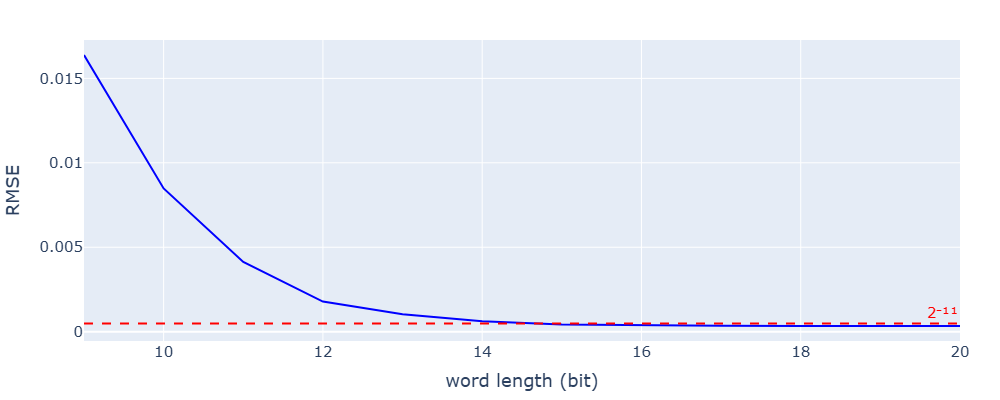
\includegraphics[width=0.8\textwidth]{../diagram/Q3/qntz_coef.png}
            \caption{Output RMSE versus coefficient word-length}
            \label{fig:qntz_coef}
        \end{figure}

        \begin{figure}[htbp]
            \centering
            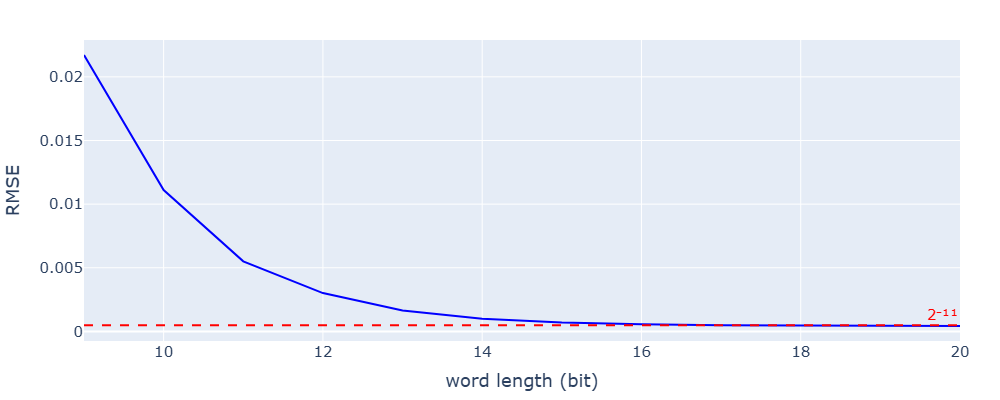
\includegraphics[width=0.8\textwidth]{../diagram/Q3/qntz_mult.png}
            \caption{Output RMSE versus multiplier word-length}
            \label{fig:qntz_mult}
        \end{figure}

        \begin{figure}[htbp]
            \centering
            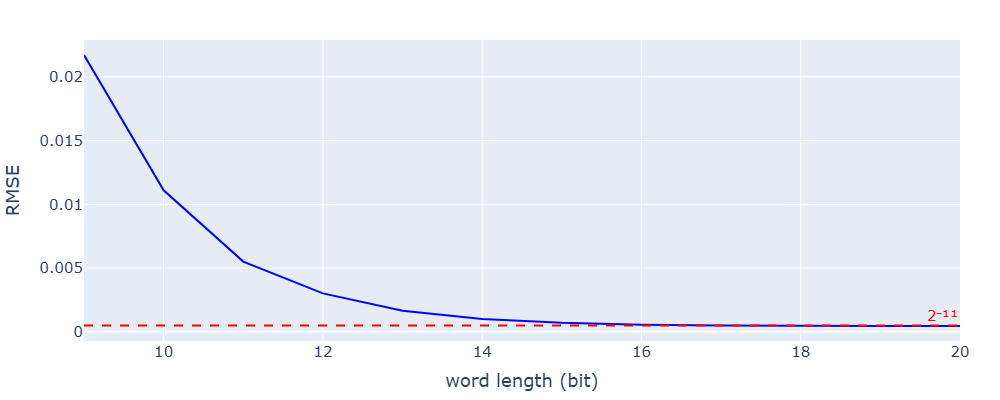
\includegraphics[width=0.8\textwidth]{../diagram/Q3/qntz_add.png}
            \caption{Output RMSE versus adder word-length}
            \label{fig:qntz_add}
        \end{figure}

        \begin{figure}[htbp]
            \centering
            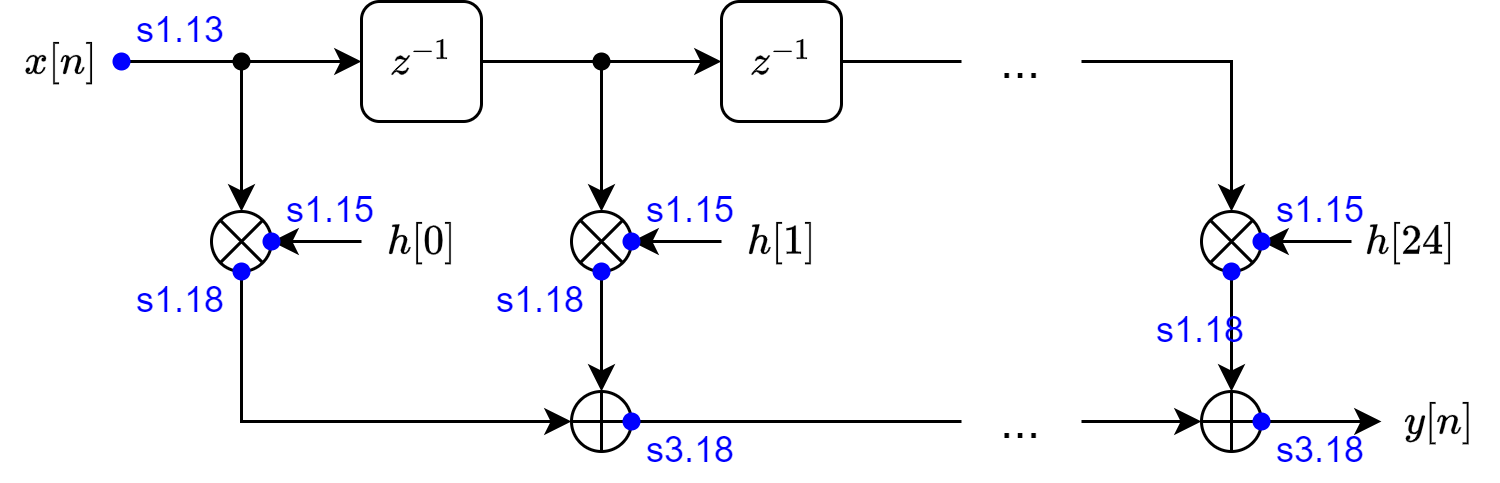
\includegraphics[width=0.8\textwidth]{../diagram/Q3/fixed_point_setting.png}
            \caption{Fixed-point setting}
            \label{fig:fixed_point_setting}
        \end{figure}

        \newpage
        \item (Step 3) Draw the fixed-point output of time domain signal. (10\%) Compare to the floating-point output and draw the error. (10\%) Show the frequency response of the fixed-point direct-form FIR filter.(10\%) Compare to the frequency response of floating-point results and draw the error of the magnitude response in passband (within 3dB bandwidth), expressed in dB (5\%)

        The time-domain fixed-point output and its error relative to the floating-point output are shown in Figures \ref{fig:output_in_time} and \ref{fig:output_error_in_time}, respectively. Although some samples exhibit relatively large errors, the overall RMSE still satisfies the specification. The frequency response of the fixed-point filter and its error compared to the floating-point counterpart are presented in Figures \ref{fig:filter_in_freq} and \ref{fig:filter_error_in_freq}, respectively. The error is on the order of several hundred micro–dB.

        \begin{figure}[htbp]
            \centering
            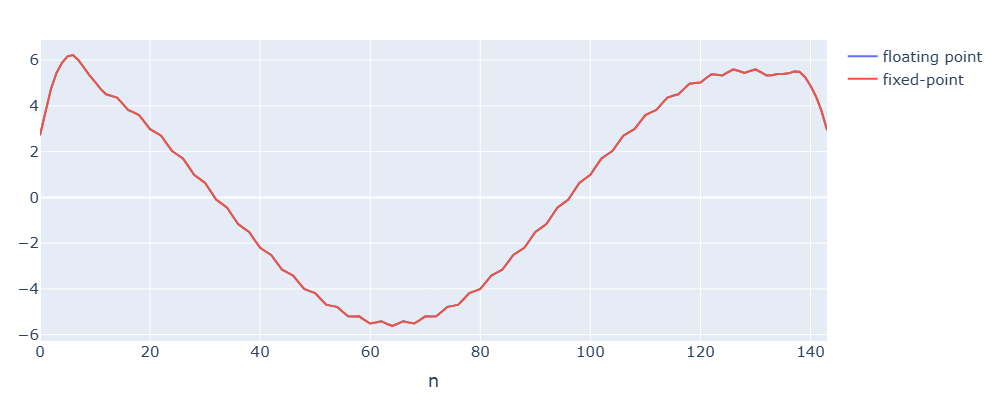
\includegraphics[width=0.8\textwidth]{../diagram/Q4/output_in_time.png}
            \caption{Time domain signal output}
            \label{fig:output_in_time}
        \end{figure}

        \begin{figure}[htbp]
            \centering
            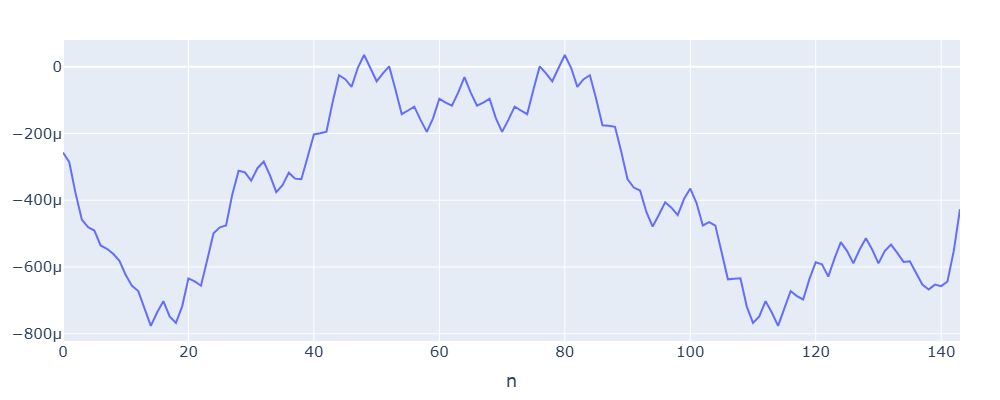
\includegraphics[width=0.8\textwidth]{../diagram/Q4/output_error_in_time.png}
            \caption{Error of time domain signal output}
            \label{fig:output_error_in_time}
        \end{figure}

        \begin{figure}[htbp]
            \centering
            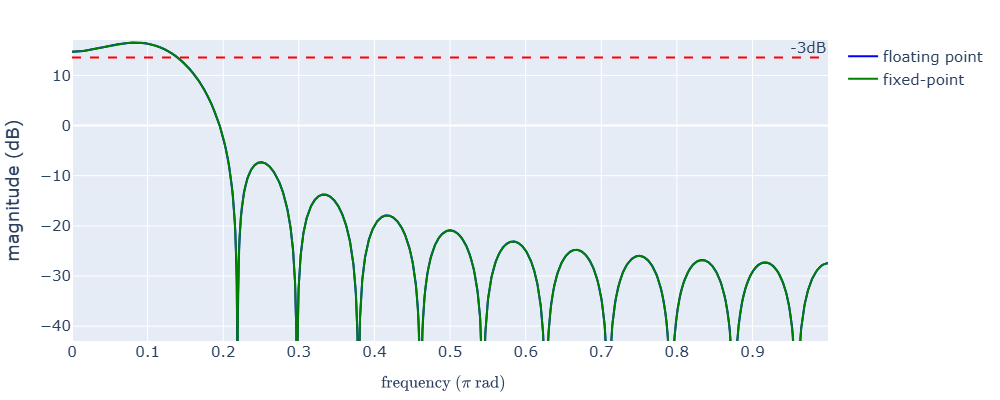
\includegraphics[width=0.8\textwidth]{../diagram/Q4/filter_in_freq.png}
            \caption{Filter frequency response}
            \label{fig:filter_in_freq}
        \end{figure}

        \begin{figure}[htbp]
            \centering
            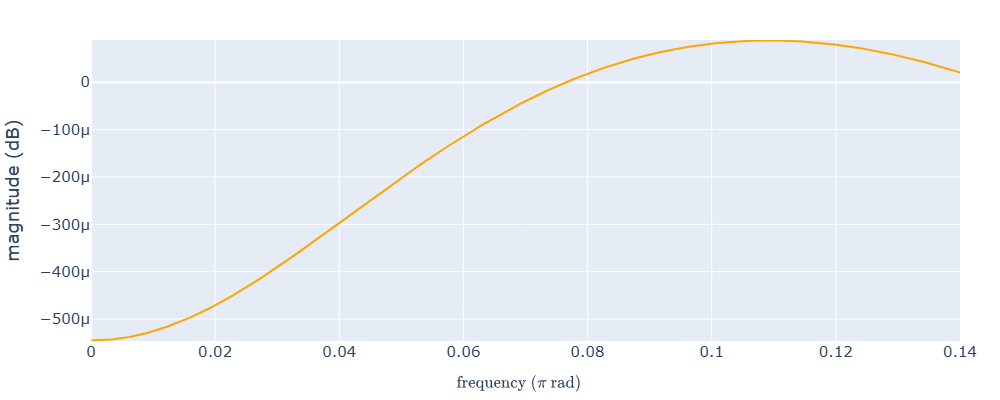
\includegraphics[width=0.8\textwidth]{../diagram/Q4/filter_error_in_freq.png}
            \caption{Error of filter frequency response within 3dB bandwidth}
            \label{fig:filter_error_in_freq}
        \end{figure}

        \newpage
        \item (Step 4) Print out the behavior timing diagram for the first 20 samples and the last 20 samples (10\%). Show the errors of hardware outputs and Matlab floating-point results of direct form FIR filter output $y[n]$ for $0\leq n\leq 143$ by figures. The latency is not constrained. (10\%)
        
        The behavioral simulation results are shown in Figures \ref{fig:behav_sim_sample_0_9}, \ref{fig:behav_sim_sample_10_19}, \ref{fig:behav_sim_sample_124_133}, and \ref{fig:behav_sim_sample_134_143}. The comparison with the floating-point output and the corresponding error are presented in Figures \ref{fig:behav_sim_output} and \ref{fig:behav_sim_output_error}, respectively.

        \begin{figure}[htbp]
            \centering
            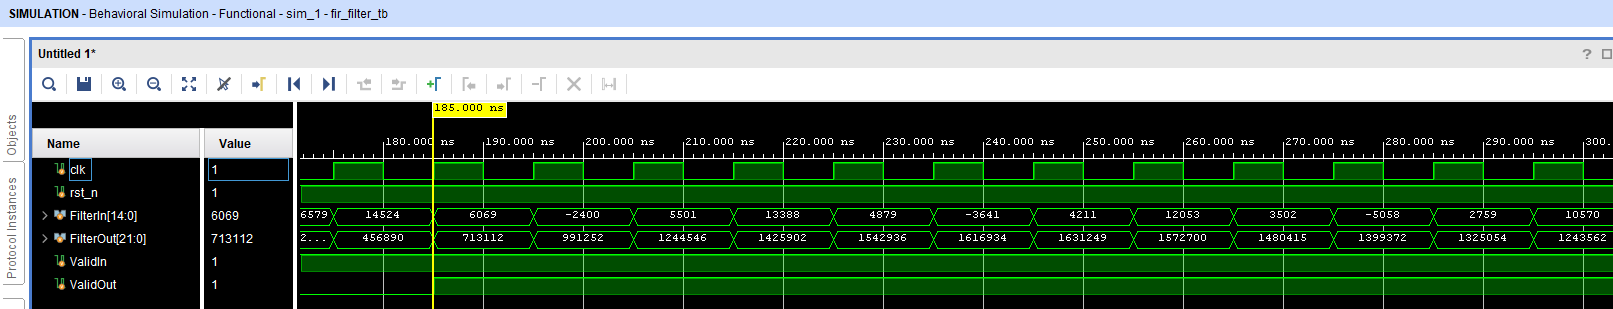
\includegraphics[width=0.8\textwidth]{../diagram/Q5/behav_sim_sample_0_9.png}
            \caption{Behavior simulation output sample 0 to 9}
            \label{fig:behav_sim_sample_0_9}
        \end{figure}

        \begin{figure}[htbp]
            \centering
            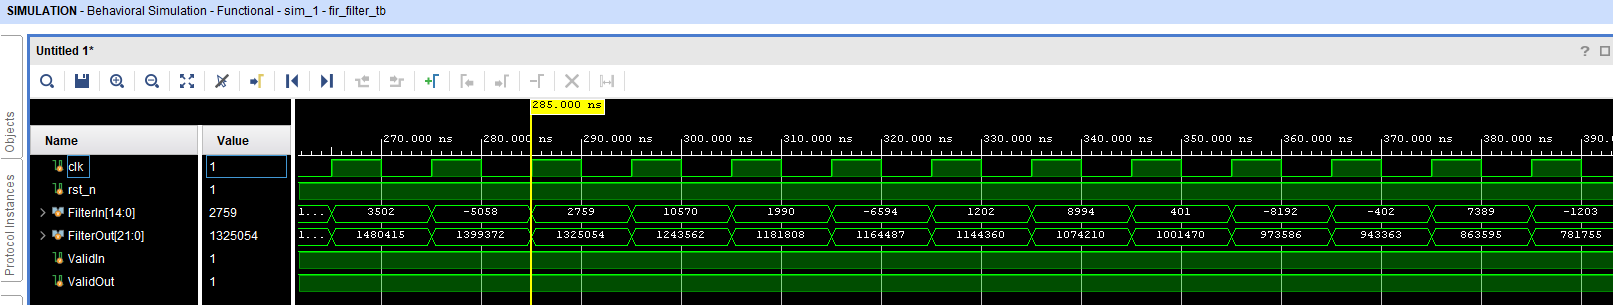
\includegraphics[width=0.8\textwidth]{../diagram/Q5/behav_sim_sample_10_19.png}
            \caption{Behavior simulation output sample 10 to 19}
            \label{fig:behav_sim_sample_10_19}
        \end{figure}

        \begin{figure}[htbp]
            \centering
            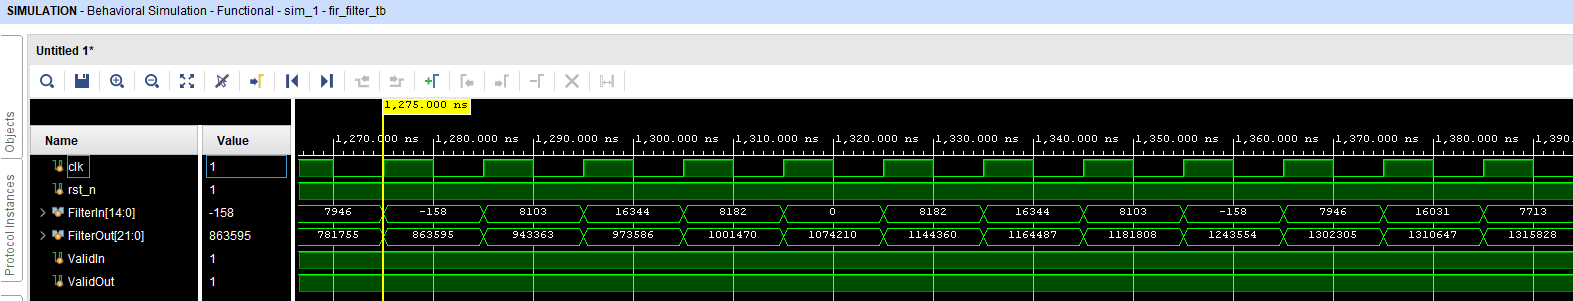
\includegraphics[width=0.8\textwidth]{../diagram/Q5/behav_sim_sample_124_133.png}
            \caption{Behavior simulation output sample 124 to 133}
            \label{fig:behav_sim_sample_124_133}
        \end{figure}

        \begin{figure}[htbp]
            \centering
            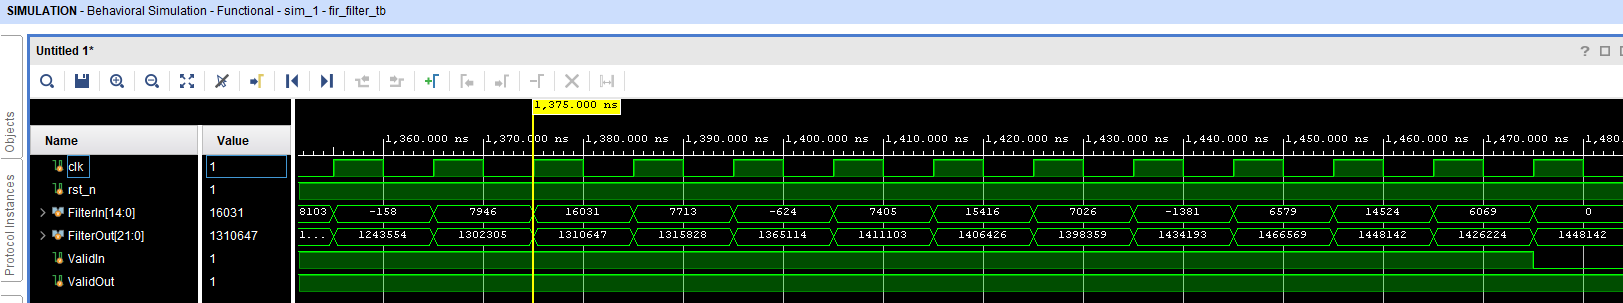
\includegraphics[width=0.8\textwidth]{../diagram/Q5/behav_sim_sample_134_143.png}
            \caption{Behavior simulation output sample 134 to 143}
            \label{fig:behav_sim_sample_134_143}
        \end{figure}

        \begin{figure}[htbp]
            \centering
            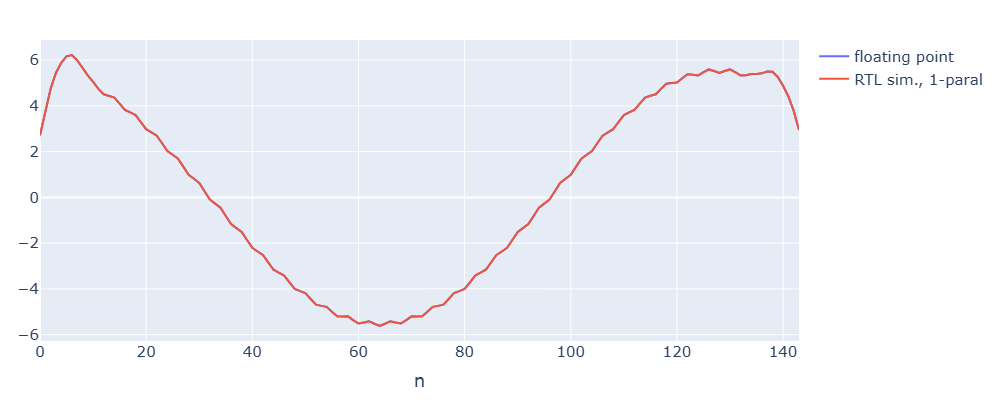
\includegraphics[width=0.8\textwidth]{../diagram/Q5/rtl_sim_paral_1.png}
            \caption{Behavior simulation output and floating point output}
            \label{fig:behav_sim_output}
        \end{figure}

        \begin{figure}[htbp]
            \centering
            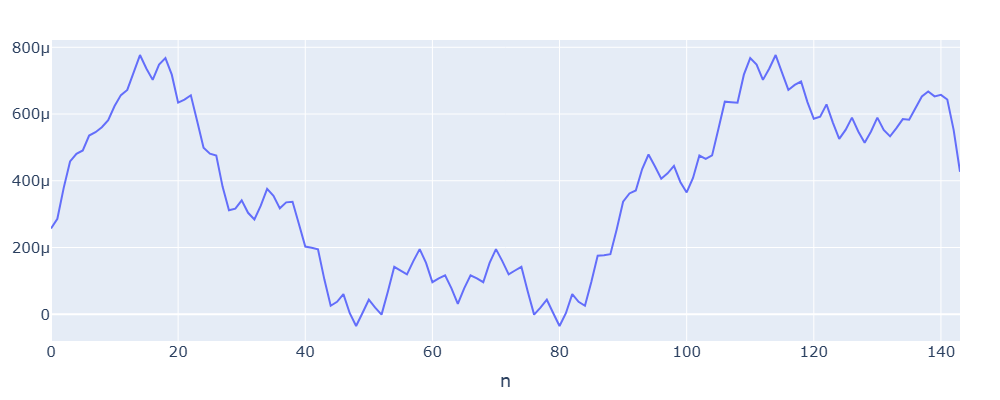
\includegraphics[width=0.8\textwidth]{../diagram/Q5/rtl_sim_paral_1_error.png}
            \caption{Behavior simulation output error (comparing to floating point)}
            \label{fig:behav_sim_output_error}
        \end{figure}

        \newpage
        \item (Step 4) Paste the timing report about the critical path. Show the numbers of adders and multipliers in the critical path. (5\%). List your timing constraint to achieve the highest operating frequency (5\%). Print out the post-SYNTHESIS timing diagram for the first 20 samples and the last 20 samples (10\%). and show the errors of post synthesis simulation outputs and Matlab floating-point results of direct-form FIR filter output $y[n]$ for $0\leq n\leq 143$ (10\%).

        The timing report and the schematic of the critical path are shown in Figures \ref{fig:critical_path_timing_report} and \ref{fig:critical_path_schematic}, respectively. Since pipeline registers are inserted between the multipliers and adders, the critical path is dominated by the accumulation stage of the FIR filter. Notably, a balanced adder tree is not employed, resulting in a summation chain structure.

        The exact number of adders on the critical path cannot be precisely determined, as the path consists of a cascaded combination of multiple adders. However, the presence of multiple levels of CARRY and LUT elements reflects this adder-chain implementation.

        A clock frequency of 100 MHz is specified as the sole timing constraint. The post-synthesis simulation results are shown in Figures \ref{fig:post_syn_sim_sample_0_9}, \ref{fig:post_syn_sim_sample_10_19}, \ref{fig:post_syn_sim_sample_124_133}, and \ref{fig:post_syn_sim_sample_134_143}. The comparison with the floating-point output and the corresponding error are presented in Figures \ref{fig:post_syn_sim_output} and \ref{fig:post_syn_sim_output_error}, respectively.

        Notably, large errors are observed at the beginning of the output, where the number of valid samples is reduced by seven. This indicates a potential issue in the post-synthesis design or timing constraints, which requires further investigation.

        \begin{figure}[htbp]
            \centering
            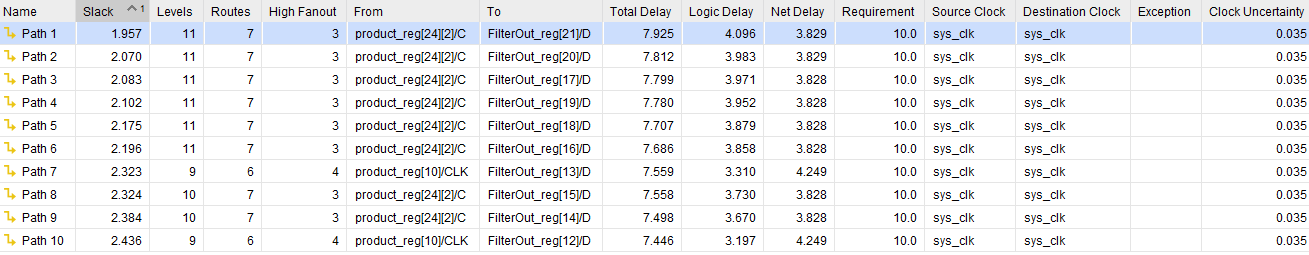
\includegraphics[width=0.8\textwidth]{../diagram/Q6/critical_path_timing_report.png}
            \caption{Timing report of critical path}
            \label{fig:critical_path_timing_report}
        \end{figure}

        \begin{figure}[htbp]
            \centering
            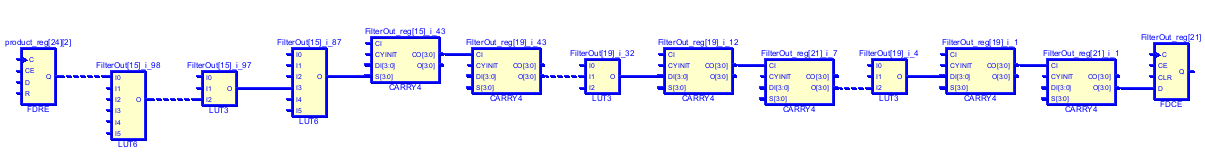
\includegraphics[width=0.8\textwidth]{../diagram/Q6/critical_path_schematic.png}
            \caption{Schematic of critical path}
            \label{fig:critical_path_schematic}
        \end{figure}

        \begin{figure}[htbp]
            \centering
            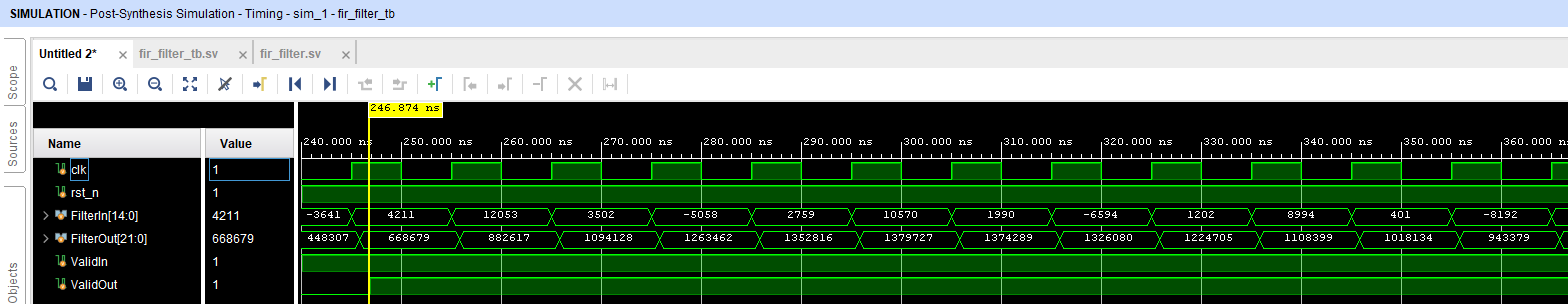
\includegraphics[width=0.8\textwidth]{../diagram/Q6/post_syn_sim_sample_0_9.png}
            \caption{Post synthesis simulation output sample 0 to 9}
            \label{fig:post_syn_sim_sample_0_9}
        \end{figure}

        \begin{figure}[htbp]
            \centering
            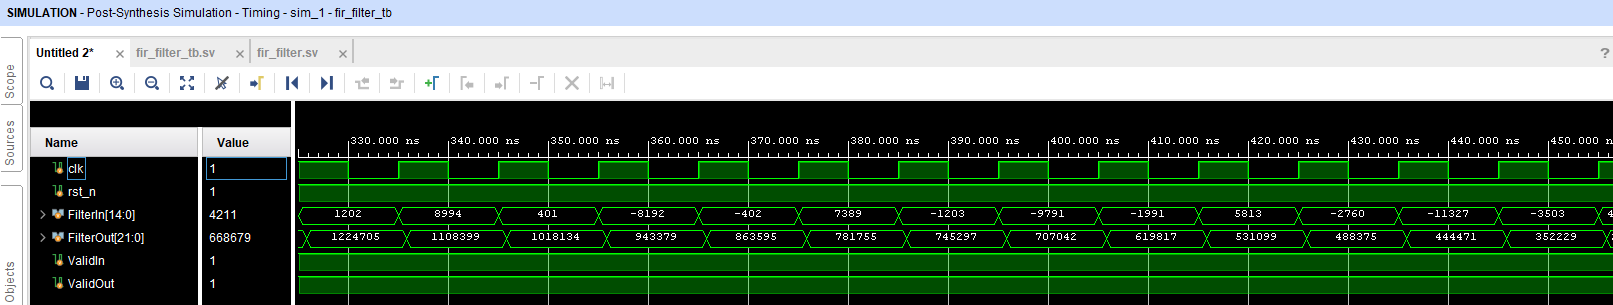
\includegraphics[width=0.8\textwidth]{../diagram/Q6/post_syn_sim_sample_10_19.png}
            \caption{Post synthesis simulation output sample 10 to 19}
            \label{fig:post_syn_sim_sample_10_19}
        \end{figure}

        \begin{figure}[htbp]
            \centering
            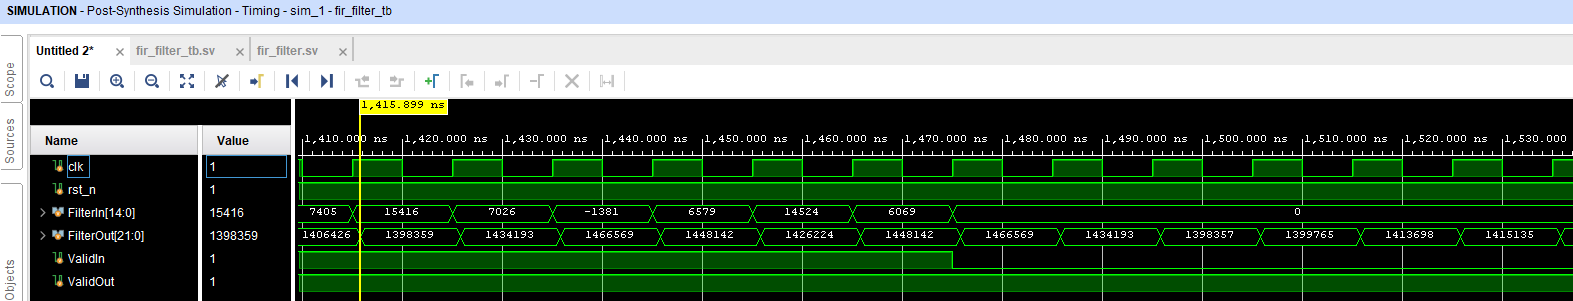
\includegraphics[width=0.8\textwidth]{../diagram/Q6/post_syn_sim_sample_124_133.png}
            \caption{Post synthesis simulation output sample 124 to 133}
            \label{fig:post_syn_sim_sample_124_133}
        \end{figure}

        \begin{figure}[htbp]
            \centering
            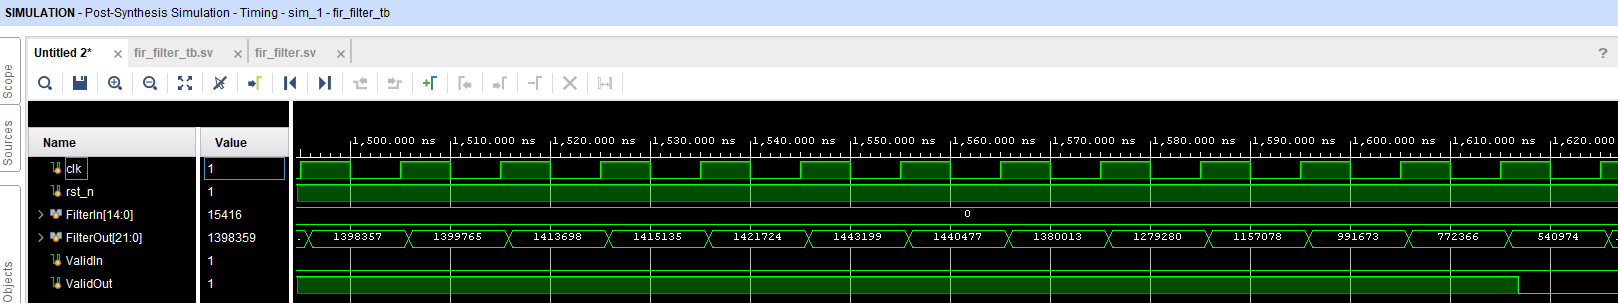
\includegraphics[width=0.8\textwidth]{../diagram/Q6/post_syn_sim_sample_134_143.png}
            \caption{Post synthesis simulation output sample 134 to 143}
            \label{fig:post_syn_sim_sample_134_143}
        \end{figure}

        \begin{figure}[htbp]
            \centering
            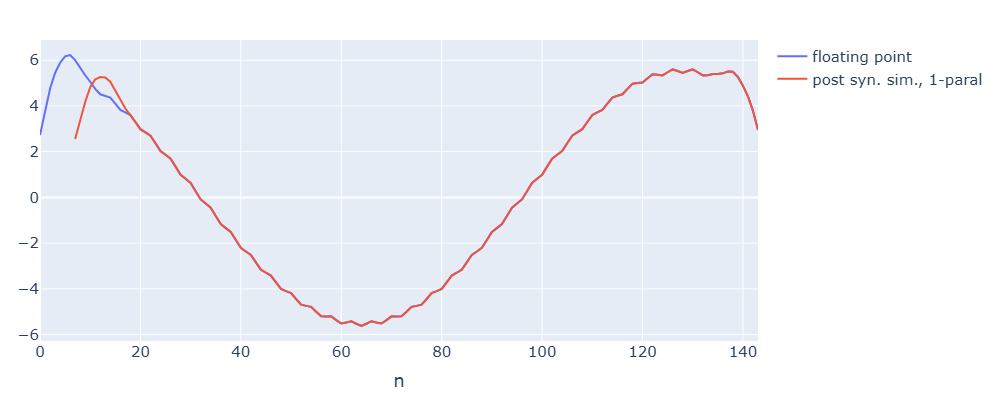
\includegraphics[width=0.8\textwidth]{../diagram/Q6/gl_sim_paral_1.png}
            \caption{Post synthesis simulation output and floating point output}
            \label{fig:post_syn_sim_output}
        \end{figure}

        \begin{figure}[htbp]
            \centering
            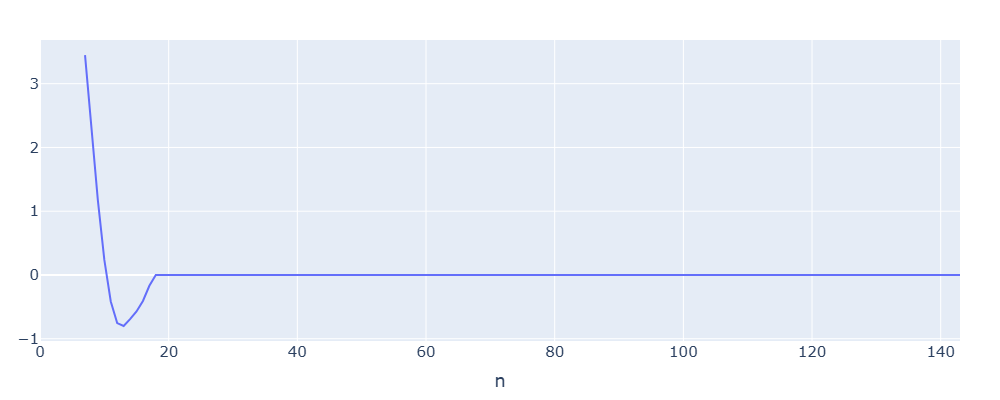
\includegraphics[width=0.8\textwidth]{../diagram/Q6/gl_sim_paral_1_error.png}
            \caption{Post synthesis simulation output error (comparing to floating point)}
            \label{fig:post_syn_sim_output_error}
        \end{figure}

        \newpage
        \item (Step 5) Show that $y[n]$ to $y[143]$ can be generated within $T_{out}/2$ in the behavior timing diagram. Draw the block diagram and indicate your critical path. (15\%). Show your synthesis report of max delay to verify your explanations. (5\%)

        The behavioral timing diagram is shown in Figure \ref{fig:output_of_2_paral}, indicating that the output can be generated within $(845 - 125)/10 = 72 = 144/2$ cycles. The block diagram in Figure \ref{fig:block_diagram_of_2_paral} shows that the parallel architecture employs the same multiplier and adder structure as the non-parallel design; therefore, the critical path remains unchanged. The synthesis report in Figure \ref{fig:critical_path_timing_report_of_2_paral} confirms that the critical path is identical to that in Figure \ref{fig:critical_path_timing_report}.

        \begin{figure}[htbp]
            \centering
            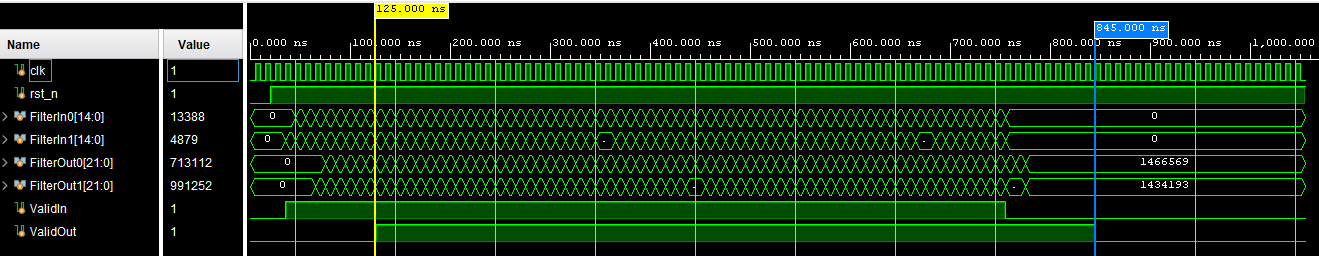
\includegraphics[width=0.8\textwidth]{../diagram/Q7/output_of_2_paral.png}
            \caption{Output of 2-parallelism}
            \label{fig:output_of_2_paral}
        \end{figure}

        \begin{figure}[htbp]
            \centering
            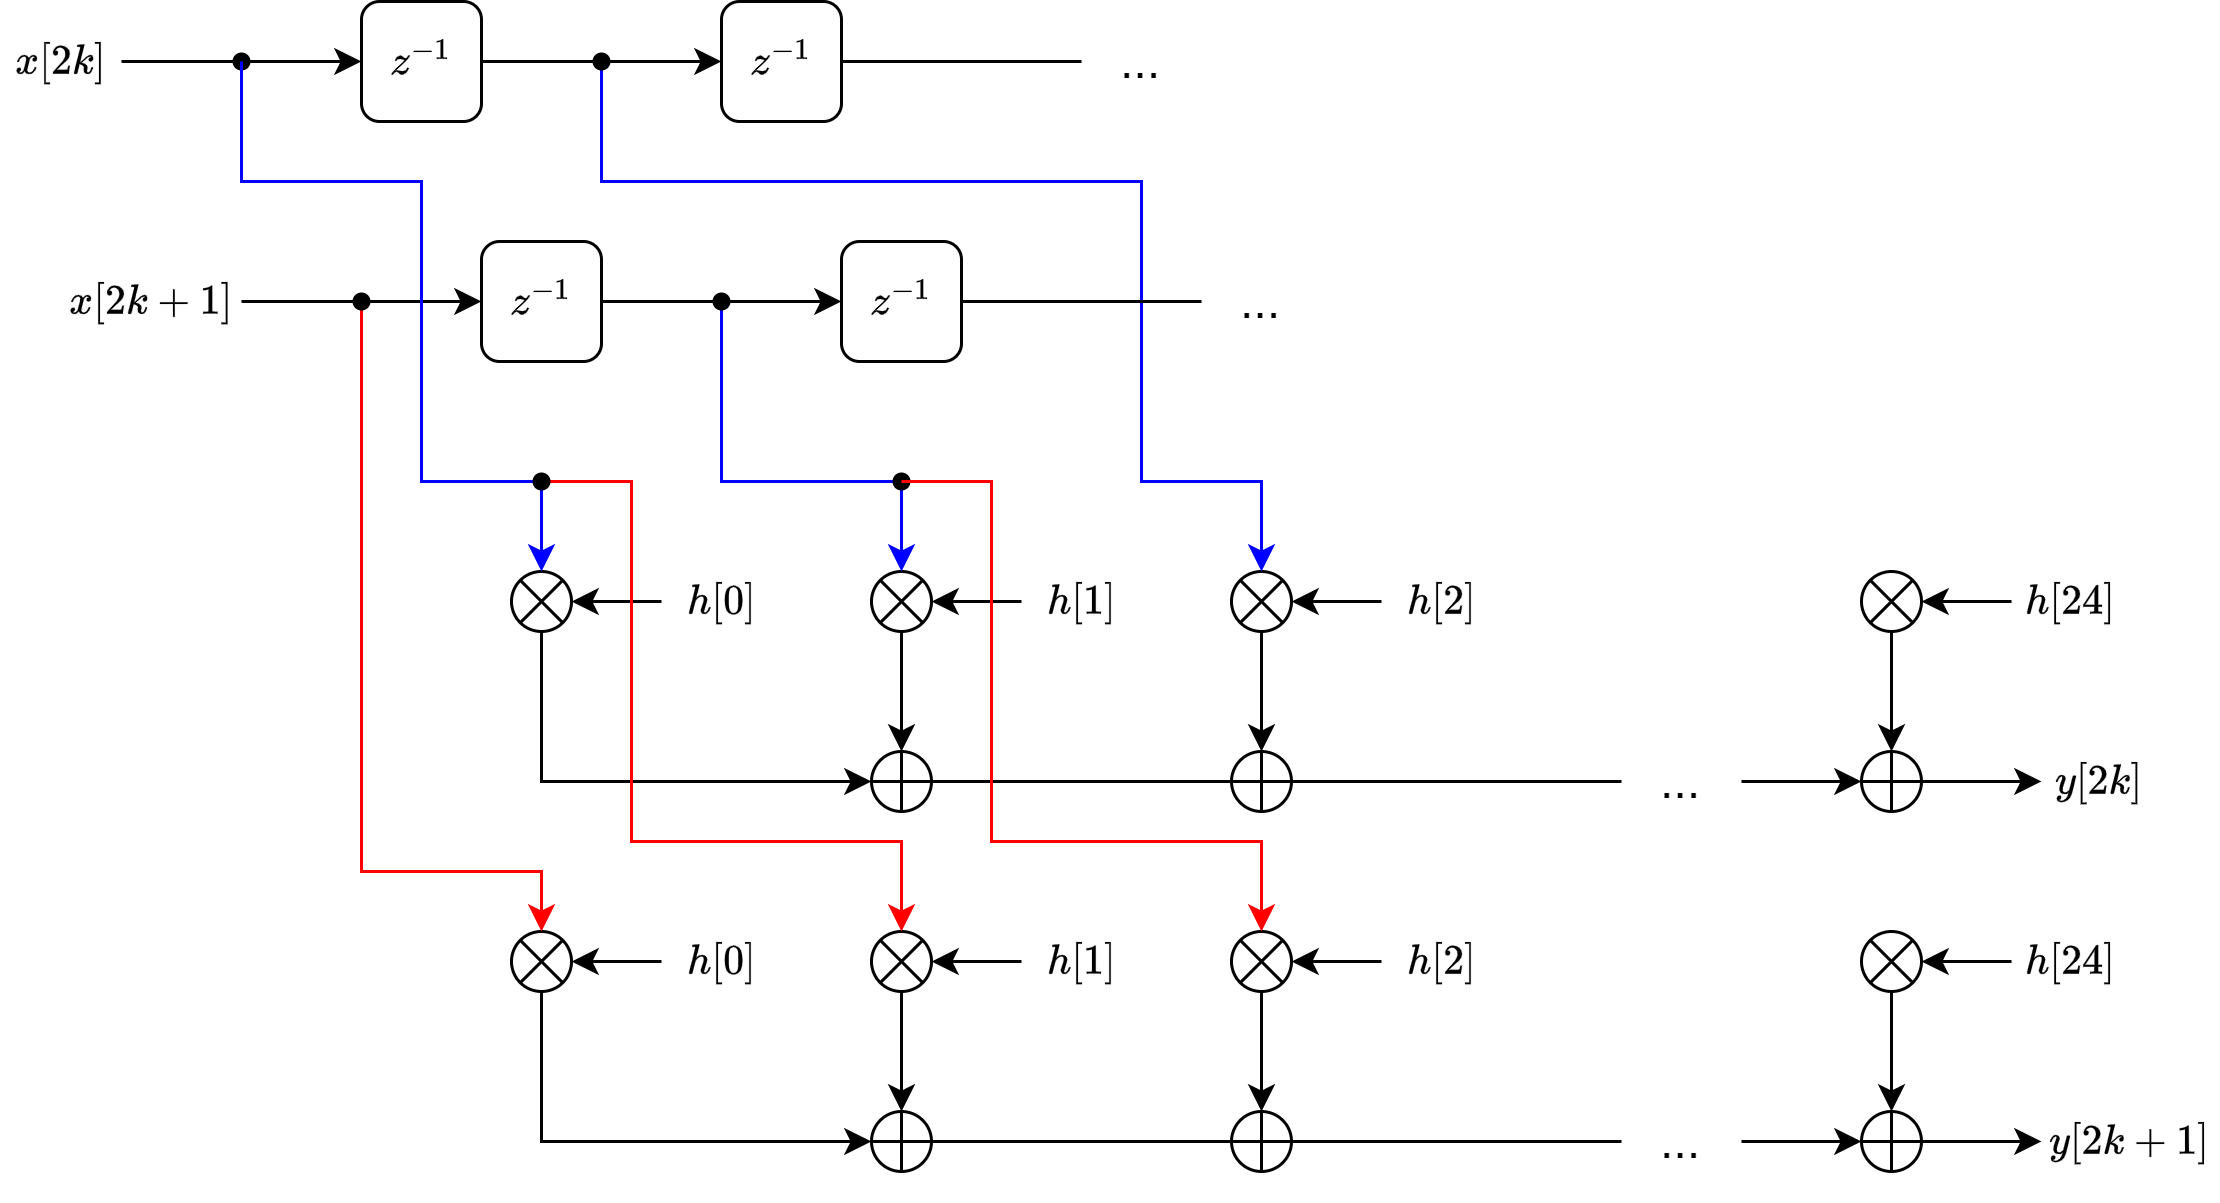
\includegraphics[width=0.8\textwidth]{../diagram/Q7/block_diagram_of_2_paral.png}
            \caption{Block diagram of 2-parallelism}
            \label{fig:block_diagram_of_2_paral}
        \end{figure}

        \begin{figure}[htbp]
            \centering
            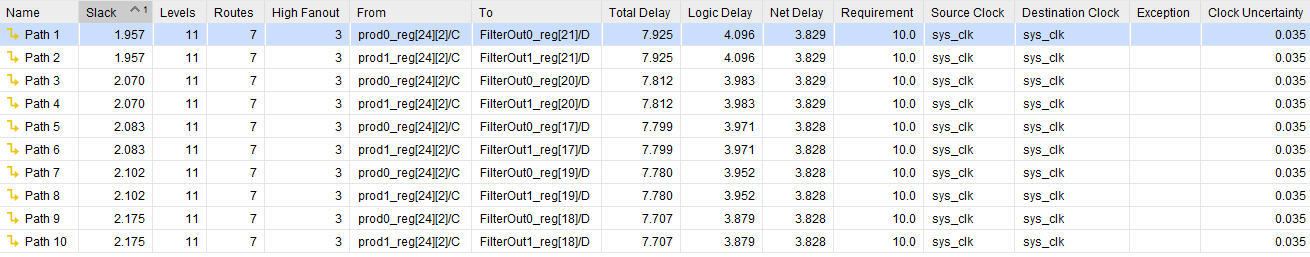
\includegraphics[width=0.8\textwidth]{../diagram/Q7/critical_path_timing_report_of_2_paral.png}
            \caption{Timing report of critical path (2-parallelism)}
            \label{fig:critical_path_timing_report_of_2_paral}
        \end{figure}

        \newpage
        \item (Step 5) Show the post-SYNTHESIS simulation results for the first 20 samples and the last 20 samples and indicate why your throughput is doubled (10\%). Show the errors of post-synthesis simulation outputs and Matlab floating-point results of direct-form FIR filter output $y[n]$ for $0\leq n\leq 143$  (10\%) Show the area (resources) before and after speedup from the synthesis report. (10\%)

        A clock frequency of 100 MHz is specified as the sole timing constraint. The post-synthesis simulation results are shown in Figures \ref{fig:post_syn_sim_sample_0_19_of_2_paral} and \ref{fig:post_syn_sim_sample_124_143_of_2_paral}. The comparison with the floating-point output and the corresponding error are presented in Figures \ref{fig:post_syn_sim_output_of_2_paral} and \ref{fig:post_syn_sim_output_error_of_2_paral}, respectively.

        Notably, large errors are observed at both the beginning and the end of the output, where the number of valid samples is reduced by fourteen. This suggests a potential issue in the post-synthesis design or timing constraints, which requires further investigation.

        The resource utilization before and after applying $2\times$ parallelism is shown in Table \ref{table:resource_usage}. The near doubling of resource usage in the 2-parallel design compared to the original is expected and reasonable.

        \begin{figure}[htbp]
            \centering
            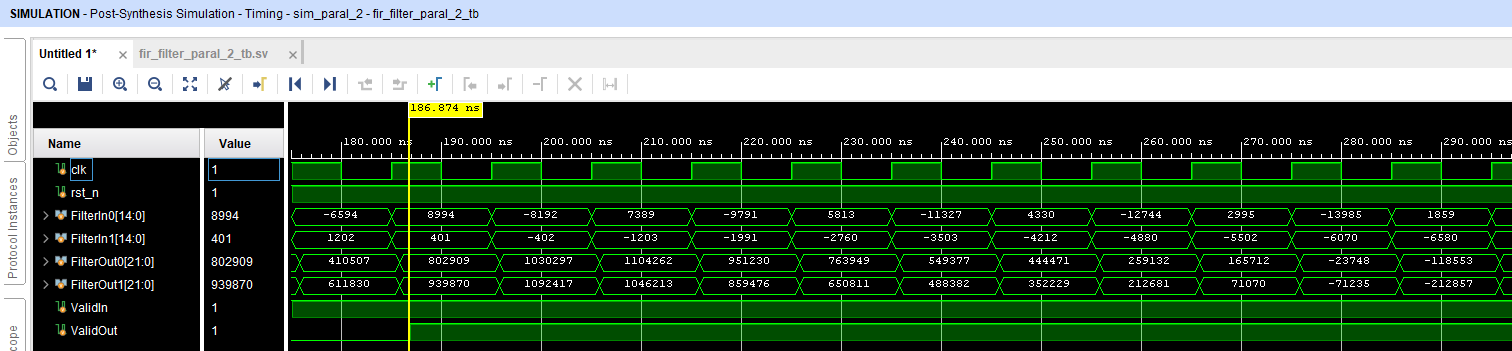
\includegraphics[width=0.8\textwidth]{../diagram/Q8/post_syn_sim_sample_0_19_of_2_paral.png}
            \caption{Post synthesis simulation output sample 0 to 19 (2-parallelism)}
            \label{fig:post_syn_sim_sample_0_19_of_2_paral}
        \end{figure}

        \begin{figure}[htbp]
            \centering
            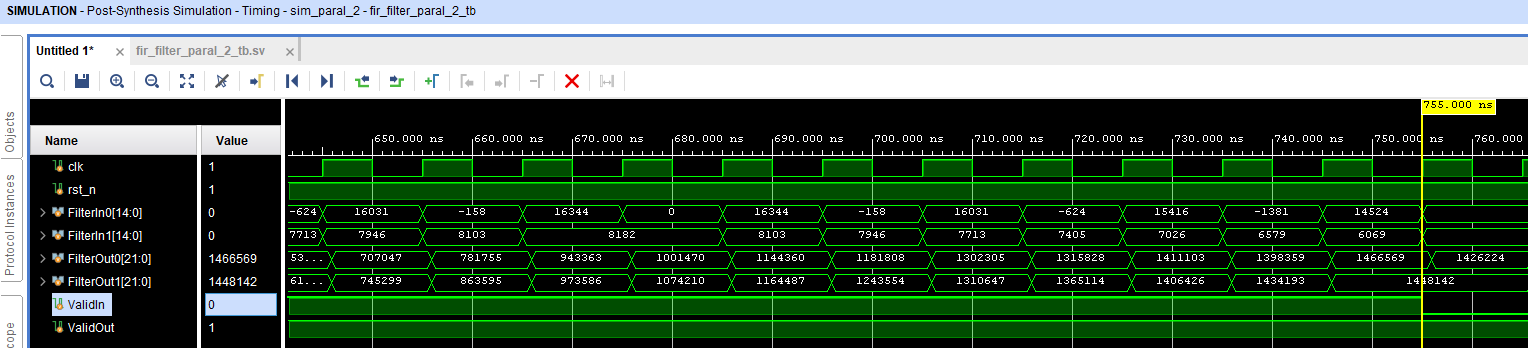
\includegraphics[width=0.8\textwidth]{../diagram/Q8/post_syn_sim_sample_124_143_of_2_paral.png}
            \caption{Post synthesis simulation output sample 124 to 143 (2-parallelism)}
            \label{fig:post_syn_sim_sample_124_143_of_2_paral}
        \end{figure}

        \begin{figure}[htbp]
            \centering
            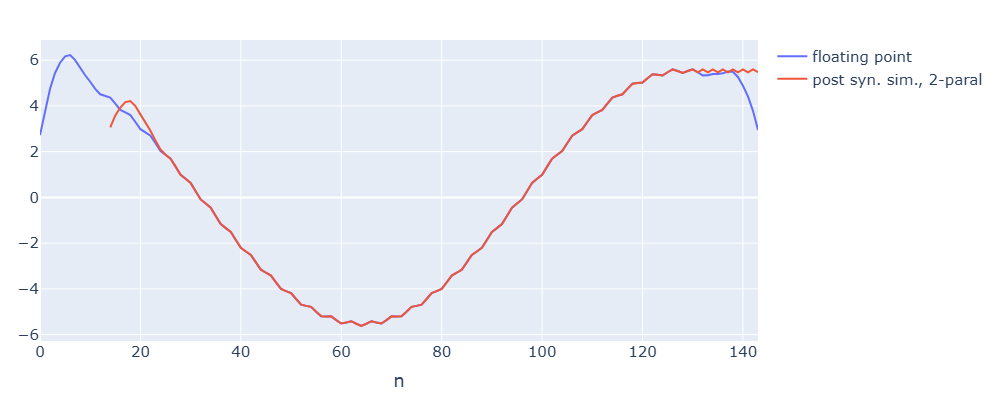
\includegraphics[width=0.8\textwidth]{../diagram/Q8/gl_sim_paral_2.png}
            \caption{Post synthesis simulation output and floating point output (2-parallelism)}
            \label{fig:post_syn_sim_output_of_2_paral}
        \end{figure}

        \begin{figure}[htbp]
            \centering
            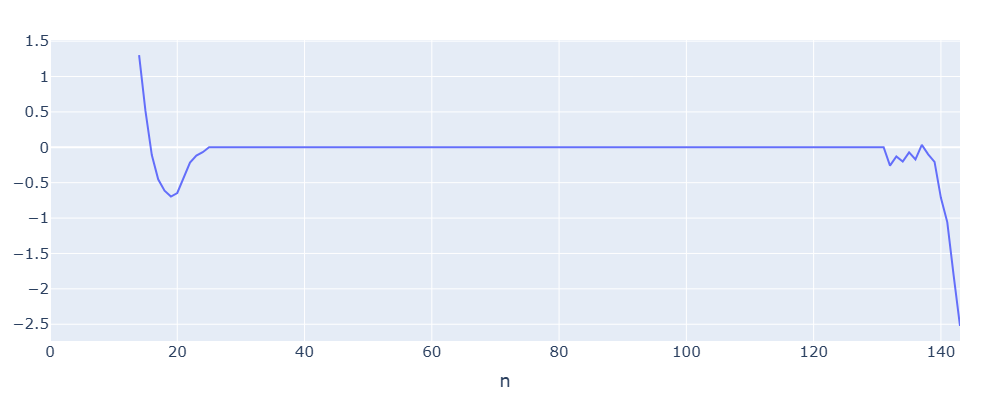
\includegraphics[width=0.8\textwidth]{../diagram/Q8/gl_sim_paral_2_error.png}
            \caption{Post synthesis simulation output error (comparing to floating point, 2-parallelism)}
            \label{fig:post_syn_sim_output_error_of_2_paral}
        \end{figure}

        \begin{table}[htbp]
        \caption{Resource utilization before and after applying $2\times$ parallelism, shown in the left and right figures, respectively.}
        \hspace*{-1.5cm}
        \begin{minipage}{0.4\textwidth}
            \centering
            \begin{verbatim}
            +----------+------+---------------------+
            | Ref Name | Used | Functional Category |
            +----------+------+---------------------+
            | FDCE     |  412 |        Flop & Latch |
            | LUT3     |  188 |                 LUT |
            | LUT6     |  149 |                 LUT |
            | CARRY4   |   80 |          CarryLogic |
            | LUT2     |   57 |                 LUT |
            | LUT1     |   31 |                 LUT |
            | FDRE     |   27 |        Flop & Latch |
            | OBUF     |   23 |                  IO |
            | LUT4     |   23 |                 LUT |
            | DSP48E1  |   20 |    Block Arithmetic |
            | IBUF     |   18 |                  IO |
            | LUT5     |    8 |                 LUT |
            | BUFG     |    1 |               Clock |
            +----------+------+---------------------+
            \end{verbatim}
        \end{minipage}
        \hspace{0.8cm}
        % --- Right Table ---
        \begin{minipage}{0.4\textwidth}
            \centering
            \begin{verbatim}
            +----------+------+---------------------+
            | Ref Name | Used | Functional Category |
            +----------+------+---------------------+
            | FDCE     |  443 |        Flop & Latch |
            | LUT3     |  376 |                 LUT |
            | LUT6     |  298 |                 LUT |
            | CARRY4   |  160 |          CarryLogic |
            | LUT2     |  114 |                 LUT |
            | LUT1     |   61 |                 LUT |
            | FDRE     |   54 |        Flop & Latch |
            | LUT4     |   46 |                 LUT |
            | OBUF     |   45 |                  IO |
            | DSP48E1  |   40 |    Block Arithmetic |
            | IBUF     |   33 |                  IO |
            | LUT5     |   16 |                 LUT |
            | BUFG     |    1 |               Clock |
            +----------+------+---------------------+
            \end{verbatim}
        \end{minipage}
        \label{table:resource_usage}
    \end{table}

\end{enumerate}

\end{document}
